\documentclass[a4paper]{article}
\usepackage[utf8]{inputenc}
\usepackage[russian]{babel}
% \usepackage[T2]{fontenc}
\usepackage[warn]{mathtext}
\usepackage{graphicx}
\usepackage{amsmath}
\usepackage{floatflt}
\usepackage[left=20mm, top=20mm, right=20mm, bottom=20mm, footskip=10mm]{geometry}


\graphicspath{ {images/} }
\usepackage{multicol}
\setlength{\columnsep}{2cm}


\begin{document}

\begin{titlepage}
	\centering
	\vspace{5cm}
	{\scshape\LARGE Московский физико-технический институт \par}
	\vspace{5cm}

	{\huge\bfseries Реферат \par}
	\vspace{1cm}
	{\scshape\Large Семестровый обзор лабораторных работ по курсу "Вакуумная Элекроника"\par}
	\vspace{1cm}
	\vfill
\begin{flushright}
	{\large выполнили студенты 852 группы ФФКЭ}\par
	\vspace{0.3cm}
	{\large Андреев Георгий} \par
	{\large Анисимов Михаил} \par
	{\large Бурков Александр} 

	
\end{flushright}
	

	\vfill

% Bottom of the page
	%Долгопрудный, 2020 г. %Я забыл нужно ли это псисать
\end{titlepage}

\section{Термоэлектронный диод}


\subsection{Цель работы}
\begin{itemize}
    \item Изготовление вакуумного диода;
    \item Измерение Вольт-Амперной характеристики диода
    \item Экспериментальная проверка справедливости формулы Ричардсона-Дэшвина и уравнения Чайлда-Ленгмюра
\end{itemize}

\subsection{Лабораторная установка}
Схема лабораторной установки для исследования характеристик термоэлектронного диода приведена на рис. 1.

\begin{figure}[h]
    \centering
    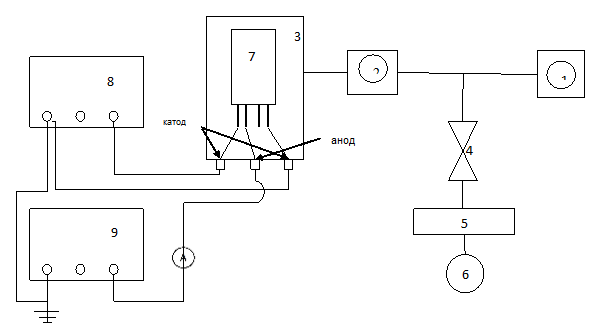
\includegraphics[width=13cm]{./Diode/setup.PNG}
    \caption{схема лабораторной установки}
    \label{fig:vac}
\end{figure}
\begin{enumerate}
    \item Форвакуумный насос
\item Турбомолекулярный насос
\item Вакуумная камера
\item Клапан с электрическим управлением
\item Измерительная насадка
\item Фильтр входящего воздуха
\item Диод
\item Источник питания HY 3010E
\item Вольтметр GPR-30H100
\end{enumerate}

\subsection{Выполнение работы}
\begin{enumerate}
    \item Осуществляем прогревание катода, параллельно снимая зависимость напряжения накала от тока накала. График зависимости приведён на рисунке 2. График зависимости сопротивления от прикладываемой мощности представлен на рисунке 3


\item Найдём зависимость температуры катода от тока накала. Температуру катода найдём из линейного приближения. Для теоретического графика зависимости температуры катода, используя закон Стефана-Больцмана.

Сравнение двух графиков представлено на рисунке 4.

\item Построим графики зависимости анодного тока от анодного напряжения в координатах $lg(I_A)$ от $lg(U_A)$ при различных значениях тока накала (рисунок 5-14)

По разным сериям экспериментов определим первеанс ($g$), отношение заряда электрона к массе ($e/m$) и эффективность катода ($\eta$). Полученные значения представлены в таблице 1.

    \begin{table}[h]
    \centering
    \begin{center}
    \caption{Данные по разным сериям экспериментов}
    \end{center}
    \vspace{0.1cm}
    \label{tab:my_label}
    \begin{tabular}{ |p{1cm}|p{1cm}|p{1cm}|p{2cm}|p{2cm}|p{2cm}|}
 \hline
 $I$, А & $U$, B & b & g & e/m, $10^{-11}$ & $\eta$, \% \\
 \hline
 \hline
2.4 & 3.7 & -1.5 & 3.13*$10^{-6}$ & 0.8 & 26.3\\
 \hline
2.5 & 3.9 & -1.39 & 3.98*$10^{-6}$ & 1.3 & 23.8\\
 \hline
2.6 & 4.1 & -1.31 & 4.88*$10^{-6}$ & 1.95 & 22.2\\
 \hline
2.7 & 4.5 & -1.18 & 6.5*$10^{-6}$ & 3.45 & 20.4 \\
 \hline
2.8 & 4.7 & -1.16 & 6.84*$10^{-6}$ & 3.84 & 19.2\\
 \hline
2.9 & 5.0 & -1.14 & 7.11*$10^{-6}$ & 4.13 & 18.2\\
 \hline 
3.0 & 5.3 & -1.12 & 7.65*$10^{-6}$ & 4.78 & 18.2\\
 \hline 

\end{tabular}
\end{table}

\end{enumerate}

\subsection{Вывод}

В ходе лабораторной работы
\begin{enumerate}
    \item Выполнен монтаж термоэлектронного диода
    \item Изученны основные характеристики диода: первеанс и эффективность;

    \item Экспериментально подтверждены закономерности ВАХ диода: При насыщении справедлив закон Ричардсона-Дэшмана, при больших токах накала выполняется закон Чайлда-Ленгмюра

    \item Снята зависимость нагрева катода от приложенного тока. Зафиксировано её совпадение с теоретической, посчитанной по формуле Стеффана-Больцмана.

\end{enumerate}


\newpage

\begin{figure}[h]
\begin{center}
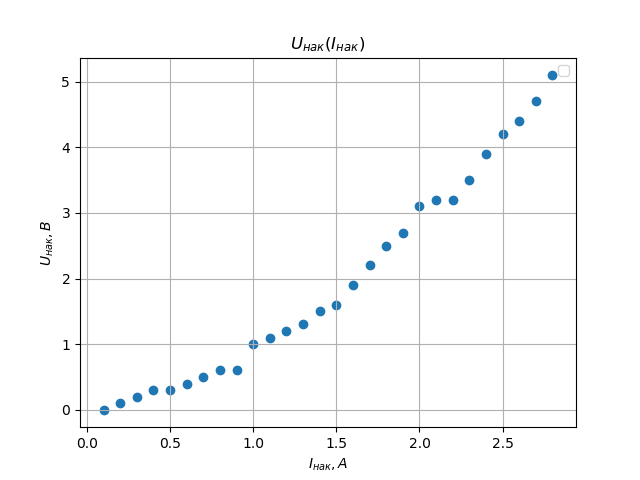
\includegraphics[width=13cm]{./Diode/fig1.PNG}
\caption{Зависимость напряжения накала от тока накала}
\label{ris:experimoriginal} %% метка рисунка для ссылки на него
\end{center}
\end{figure}

\begin{figure}[h]
\begin{center}
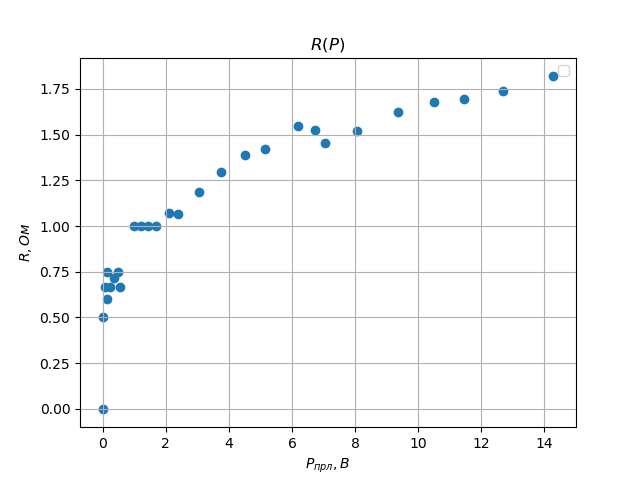
\includegraphics[width=13cm]{./Diode/fig2.PNG}
\caption{Зависимость сопротивления катода от приложенной мощности}
\label{ris:experimoriginal} %% метка рисунка для ссылки на него
\end{center}
\end{figure}

\begin{figure}[h]
\begin{center}
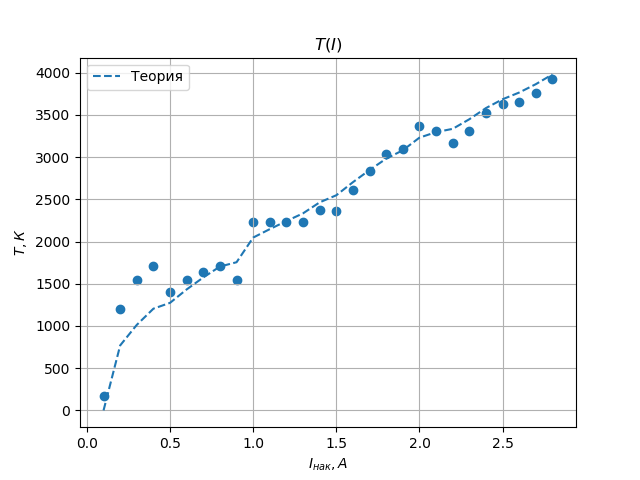
\includegraphics[width=13cm]{./Diode/fig3.PNG}
\caption{Зависимость температуры катода от тока накала: расчёт по измерению сопротивления и по уравнению Стефана-Больцмана}
\label{ris:experimoriginal} %% метка рисунка для ссылки на него
\end{center}
\end{figure}

\begin{figure}[h]
\begin{center}
\begin{minipage}[h]{0.45\linewidth}
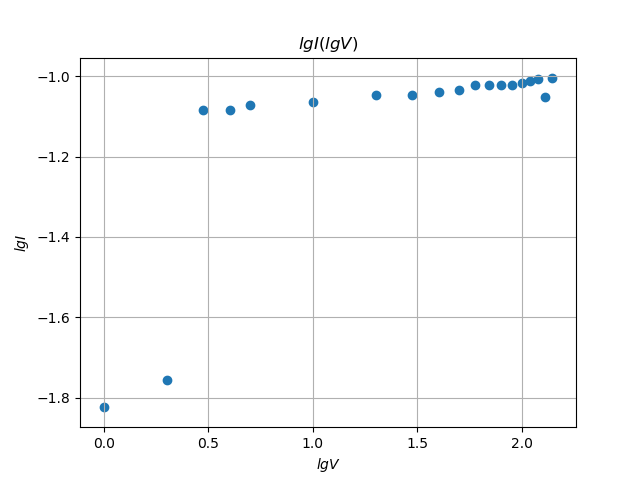
\includegraphics[width=1\linewidth]{./Diode/graph_1.png}
\caption{Зависимость $lg(I_A)$ от $lg(V_A)$ при токе накала 2.3 А, напряжении накала 3.4 B} %% подпись к рисунку\label{ris:experimoriginal} %% метка рисунка для ссылки на него
\end{minipage}
\hfill 
\begin{minipage}[h]{0.45\linewidth}
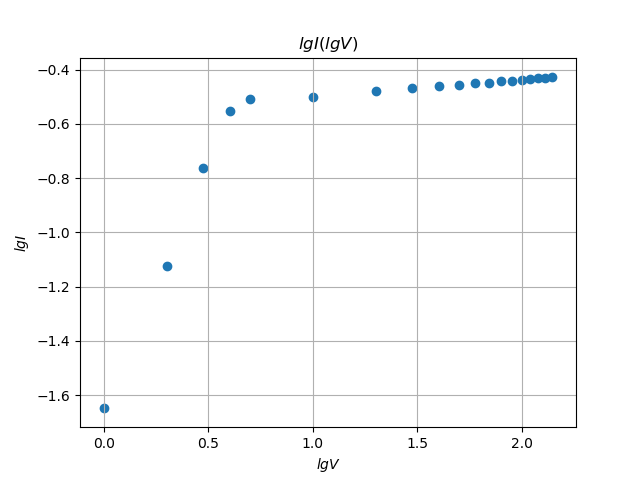
\includegraphics[width=1\linewidth]{./Diode/graph_2.png}
\caption{Зависимость $lg(I_A)$ от $lg(V_A)$ при токе накала 2.4 А, напряжении накала 3.7 B }
\label{ris:experimcoded}
\end{minipage}
\end{center}
\end{figure}

\begin{figure}[h]
\begin{center}
\begin{minipage}[h]{0.45\linewidth}
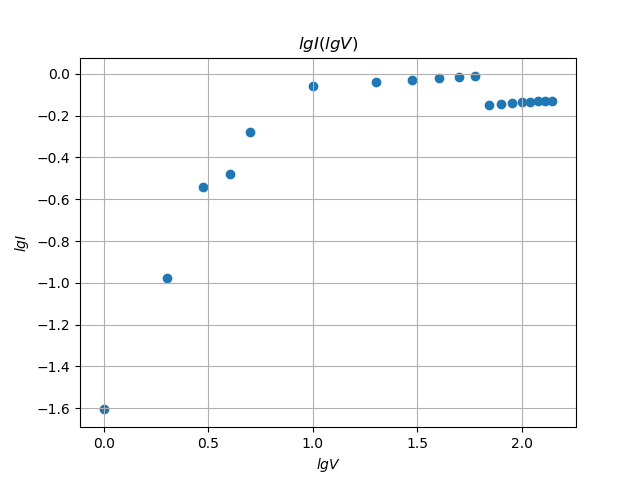
\includegraphics[width=1\linewidth]{./Diode/graph_3.png}
\caption{Зависимость $lg(I_A)$ от $lg(V_A)$ при токе накала 2.5 А, напряжении накала 3.9 B} %% подпись к рисунку\label{ris:experimoriginal} %% метка рисунка для ссылки на него
\end{minipage}
\hfill 
\begin{minipage}[h]{0.45\linewidth}
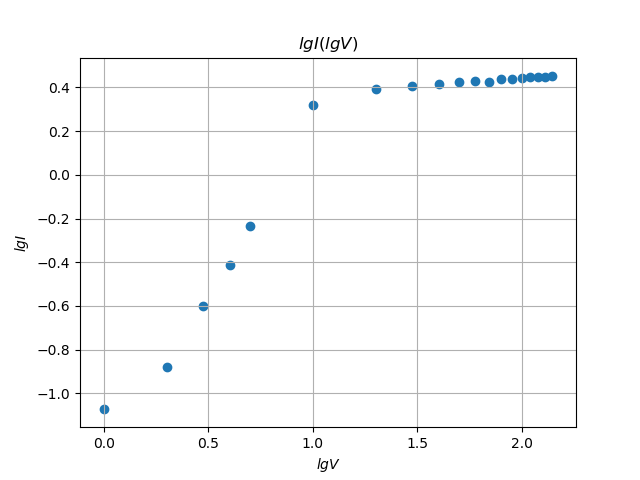
\includegraphics[width=1\linewidth]{./Diode/graph_4.png}
\caption{Зависимость $lg(I_A)$ от $lg(V_A)$ при токе накала 2.6 А, напряжении накала 4.1 B }
\label{ris:experimcoded}
\end{minipage}
\end{center}
\end{figure}

\begin{figure}[h]
\begin{center}
\begin{minipage}[h]{0.45\linewidth}
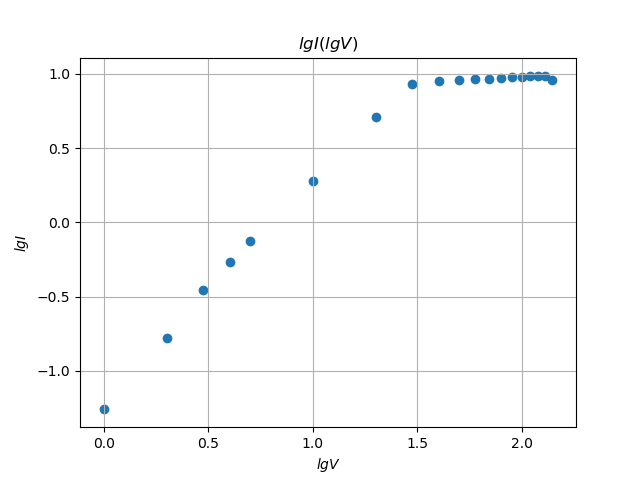
\includegraphics[width=1\linewidth]{./Diode/graph_5.png}
\caption{Зависимость $lg(I_A)$ от $lg(V_A)$ при токе накала 2.7 А, напряжении накала 4.5 B} %% подпись к рисунку\label{ris:experimoriginal} %% метка рисунка для ссылки на него
\end{minipage}
\hfill 
\begin{minipage}[h]{0.45\linewidth}
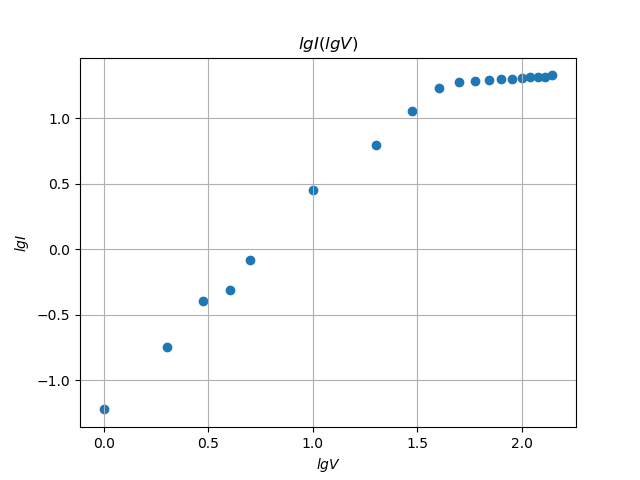
\includegraphics[width=1\linewidth]{./Diode/graph_6.png}
\caption{Зависимость $lg(I_A)$ от $lg(V_A)$ при токе накала 2.8 А, напряжении накала 4.7 B }
\label{ris:experimcoded}
\end{minipage}
\end{center}
\end{figure}


\begin{figure}[h]
\begin{center}
\begin{minipage}[h]{0.45\linewidth}
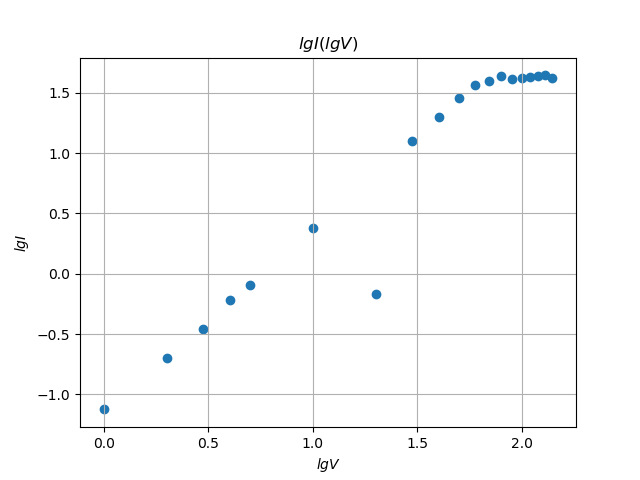
\includegraphics[width=1\linewidth]{./Diode/graph_7.png}
\caption{Зависимость $lg(I_A)$ от $lg(V_A)$ при токе накала 2.9 А, напряжении накала 5.0 B }
\label{ris:experimcoded}
\end{minipage}
\hfill 
\begin{minipage}[h]{0.45\linewidth}
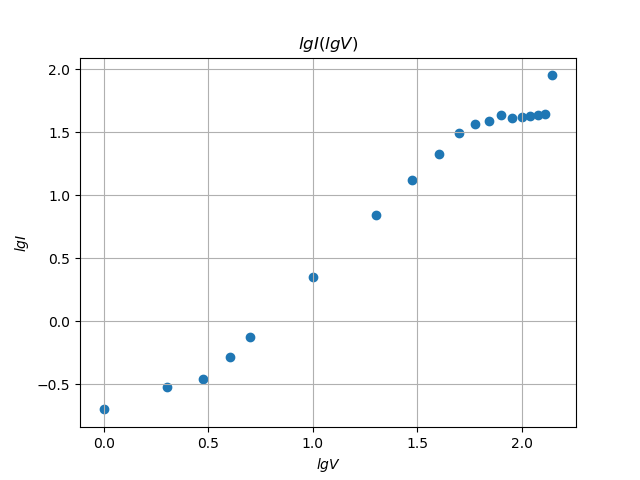
\includegraphics[width=1\linewidth]{./Diode/graph_8.png}
\caption{Зависимость $lg(I_A)$ от $lg(V_A)$ при токе накала 3.0 А, напряжении накала 5.3 B }
\label{ris:experimcoded}
\end{minipage}
\end{center}
\end{figure}


\begin{figure}[h]
\begin{center}
\begin{minipage}[h]{0.45\linewidth}
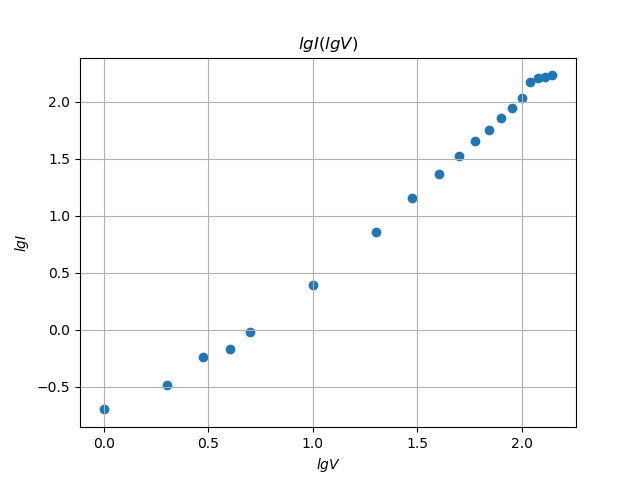
\includegraphics[width=1\linewidth]{./Diode/graph_9.png}
\caption{Зависимость $lg(I_A)$ от $lg(V_A)$ при токе накала 3.1 А, напряжении накала 5.7 B }
\label{ris:experimcoded}
\end{minipage}
\hfill 
\begin{minipage}[h]{0.45\linewidth}
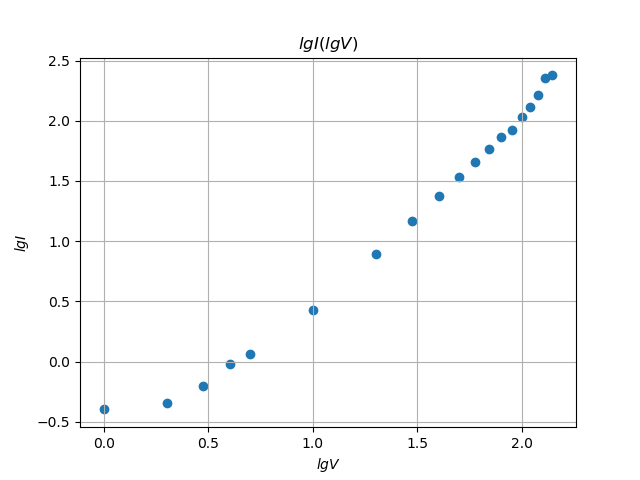
\includegraphics[width=1\linewidth]{./Diode/graph_10.png}
\caption{Зависимость $lg(I_A)$ от $lg(V_A)$ при токе накала 3.2 А, напряжении накала 5.9 B }
\label{ris:experimcoded}
\end{minipage}
\end{center}
\end{figure}


\end{document}
